% 45 min d'exposé en français (questions incluses)

% ajouter arbres au début

\documentclass[slidetop,11pt %, aspectratio=1610
]{beamer}

\usepackage[T1]{fontenc} 
\usepackage[utf8]{inputenc}
\usepackage[ english,french]{babel}
\usepackage{lmodern}
\usepackage{aeguill}
\usepackage{graphics,graphicx}
\usepackage{tikz}
\usetikzlibrary{shapes, backgrounds,fit,shapes, arrows,chains,matrix,positioning,scopes, calc}
\usepackage{tikz-cd}
\usepackage{ulem}
\usepackage{frcursive}
\usepackage{array}
\usepackage{amsthm, amssymb}
\usepackage{stmaryrd}
\usepackage{todonotes}
\usepackage{xcolor, colortbl}
\usepackage{bussproofs}
\usepackage{fontawesome}
\newcolumntype{M}[1]{>{\centering\arraybackslash}m{#1}}
\usetikzlibrary{trees,shapes, positioning}
\usepackage{listings}
\lstset{language=caml}

%\newtheorem{thm}{Theorème}
%\newtheorem{lem}[theorem]{Lemme}
%\newtheorem{cor}[theorem]{Corollaire}
%\newtheorem{prop}[theorem]{Proposition}
%\theoremstyle{definition}
%\newtheorem{conj}[theorem]{Conjecture}
%\newtheorem{defi}[theorem]{Définition}
%\newtheorem{exple}[theorem]{Exemples}

%% En anglais
\newtheorem{thm}{Theorem}
\newtheorem{lem}[theorem]{Lemma}
\newtheorem{cor}[theorem]{Corollary}
\newtheorem{prop}[theorem]{Proposition}
\theoremstyle{definition}
\newtheorem{conj}[theorem]{Conjecture}
\newtheorem{defi}[theorem]{Definition}
\newtheorem{exple}[theorem]{Examples}


\usepackage{xargs}
\definecolor{Bleu}{HTML}{3333b3}
%\beamertemplatetransparentcovered

\usetheme{Boadilla}

\setbeamertemplate{navigation symbols}{} % enlever les symboles de navigation

\setbeamercolor{section in head/foot}{bg = white, fg=blue}
% aussi section in toc

\usepackage{xkeyval}

% couleurs été
%\newcommand{\coula}{6DA3B9}
%\newcommand{\coulb}{D0B080}
%\newcommand{\coulc}{254D62}
%\newcommand{\could}{8D7050}

% couleurs Cetraro
%\newcommand{\could}{590C3E}
%\newcommand{\coula}{8C2066}
%\newcommand{\coulc}{D94E81}
%\newcommand{\coulb}{BF920B}

% couleurs automne
% D4AB31
%E47127
%BC322C
% 00FA9A

%\newcommand{\coula}{D4AB31}
%\newcommand{\coulb}{E47127}
%\newcommand{\coulc}{BC322C}
%\newcommand{\could}{00FA9A}
%
% couleurs printemps
%\newcommand{\coula}{5AC1C9}
%\newcommand{\coulb}{DE5D83}
%\newcommand{\coulc}{9966CC}
%\newcommand{\could}{6698FF}

% couleurs Peps
\newcommand{\coula}{0785F2}
\newcommand{\coulb}{F29F05}
\newcommand{\coulc}{F21313}
\newcommand{\could}{E6F21F}



\definecolor{part1}{HTML}{\coula}
\definecolor{part2}{HTML}{\coulb}
\definecolor{part3}{HTML}{\coulc}
\definecolor{part4}{HTML}{\could}




\definecolor{newSec}{HTML}{\coula}
\definecolor{mauve}{HTML}{9966CC}% rouge foncé D4AB31
\definecolor{rose}{HTML}{DE5D83}
\definecolor{bleu}{HTML}{5AC1C9}%orange %{6698FF} % E47127
\definecolor{vert}{HTML}{BC322C} %vert : 5AC1C9 % 3CB371
\definecolor{quatre}{HTML}{F4C2C2}\setbeamercolor{title}{fg=newSec}
\setbeamercolor{structure}{fg=newSec}

\tikzset{
    flower/.pic = {
\shade[ball color = newSec!40,top color=newSec!10, bottom color=newSec!30] (0,0) circle (0.25cm);
  \draw[newSec] (0,0) circle (0.25cm);
  \draw[newSec] (-0.25,0) arc (180:360:0.25 and 0.075);
  \draw[dashed, newSec] (0.25,0) arc (0:180:0.25 and 0.075);


      },
}

\tikzset{
    centre/.pic = {
         \draw[white] (0,0.2) rectangle(0.1,-0.2);
%         \filldraw[fill=newSec!70, draw=black!30, rotate=\a] (0.2,0) ellipse(0.2 and 0.075);
       \filldraw[draw=newSec!70, top color=newSec!10, bottom color=newSec!30] (0,0) circle(0.1);
    },
}

\setbeamertemplate{section in head/foot}{%
    \if\insertsectionheadnumber1
%flower, fill=pink, draw=purple
        \tikz\node[circle, fill=newSec!50, draw=newSec]{\textcolor{white}{\thesection}};
%\tikz\pic{flower};
    \else
        \tikz\node[circle, fill=newSec!50, draw=newSec]{\textcolor{white}{\thesection}};
%\tikz\pic{flower};
  \fi
}

\setbeamertemplate{section in head/foot shaded}{%
    \if\insertsectionheadnumber1
%        \tikz\node[circle, fill=white, draw=gray!30]{\hskip.3cm};
        \tikz\pic{centre};
    \else
%        \tikz\node[circle, fill=white, draw=gray!30]     {\hskip.3cm};
                \tikz\pic{centre};
  \fi
}

\setbeamertemplate{headline}
{
  \leavevmode%
  \hbox{%
  \begin{beamercolorbox}[wd=\paperwidth,ht=2.5ex,dp=1.5ex,center]{section in head/foot}%
    \usebeamerfont{section in head/foot}
    \vspace*{-0.5cm}   
    \hspace{9.5cm} %%% ici pour modifier la position des sections dans le titre
    \insertsectionnavigationhorizontal{1cm}{\hskip.1cm}{}
  \end{beamercolorbox}}%
  \vskip0pt%
}


\setbeamertemplate{footline}{}

\AtBeginSection[]{ % un petit sommaire au début de chaque section
{
  \if\thesection1
     \definecolor{newSec}{HTML}{\coula}
  \else  \if\thesection2
            \definecolor{newSec}{HTML}{\coulb}
         \else \if\thesection3
                  \definecolor{newSec}{HTML}{\coulc} % 3CB371
               \else \if\thesection4
                        \definecolor{newSec}{HTML}{\could}
                      \else
                        \definecolor{newSec}{RGB}{0,255,0}
                      \fi
               \fi
         \fi
  \fi
\setbeamercolor{title}{fg=newSec}
\setbeamercolor{frametitle}{fg=newSec}
\setbeamercolor{structure}{fg=newSec}


\setbeamercolor{background canvas}{bg=newSec}
\setbeamercolor{section in head/foot}{bg = newSec}
\setbeamertemplate{headline}
{
  \leavevmode%
  \hbox{%
  \begin{beamercolorbox}[wd=\paperwidth,ht=2.5ex,dp=1.5ex,center]{section in head/foot}%
  \end{beamercolorbox}}%
  \vskip0pt%
}

  \begin{frame}{}
  
  \begin{center}
  \textcolor{white}{
  \if\thesection1
{     \LARGE \nameref{sect1}}
  \else  \if\thesection2
{     \LARGE \nameref{sect2}}
         \else \if\thesection3
{     \LARGE \nameref{sect3}}
               \else \if\thesection4
{     \LARGE \nameref{sect4}}
                      \fi
               \fi
         \fi
  \fi}
\end{center}
\end{frame} 
 
  \setbeamercolor{background canvas}{bg=}
\setbeamercolor{section in head/foot}{bg = white}  
  
%  \begin{frame}{Outline}
%  \small \tableofcontents[currentsection, hidesubsections, subsubsectionstyle=hide]
%  \addtocounter{framenumber}{-1}
%  \end{frame} 
}
  \if\thesection1
     \definecolor{newSec}{HTML}{D4AB31}
  \else  \if\thesection2
            \definecolor{newSec}{HTML}{DE5D83}
         \else \if\thesection3
                  \definecolor{newSec}{HTML}{E47127}
               \else \if\thesection4
                        \definecolor{newSec}{HTML}{F4C2C2}
                      \else
                        \definecolor{newSec}{RGB}{0,255,0}
                      \fi
               \fi
         \fi
  \fi
  
  \if\thesection1
     \definecolor{newSec}{HTML}{\coula}
  \else  \if\thesection2
            \definecolor{newSec}{HTML}{\coulb}
         \else \if\thesection3
                  \definecolor{newSec}{HTML}{\coulc}
               \else \if\thesection4
                        \definecolor{newSec}{HTML}{\could}
                      \else
                        \definecolor{newSec}{RGB}{0,255,0}
                      \fi
               \fi
         \fi
  \fi
  
\setbeamercolor{title}{fg=newSec}
\setbeamercolor{frametitle}{fg=newSec}
\setbeamercolor{structure}{fg=newSec}
 }

\setlength{\columnseprule}{0.4pt}

%\usepackage{marvosym}



\usepackage{mathabx}

% ----------- Contenu de la page de titre --------
\title{\LARGE De la diagonale du permutoèdre aux arbres k-colorés : \\ \Large une histoire de partitions et d'arbres \vspace{-0.5cm}}

\institute[IMAG - UMontpellier]{
\includegraphics[height=1.5cm]{imag.png}
\hspace{1cm}

\includegraphics[height=1.5cm]{UM.png}
\vspace{-0.3cm}
}

\begin{document}

\author[B. Delcroix-Oger]{\textcolor{part2}{Bérénice Delcroix-Oger} \\
\footnotesize
\vspace{0.5cm}
joint work with 
\begin{tabular}{l}
\textcolor{part2}{Matthieu Josuat-Vergès} (IRIF), \\
\textcolor{part2}{ Guillaume Laplante-Anfossi} (Univ. Melbourne), \\
\textcolor{part2}{ Vincent Pilaud} (LIX),\\
\textcolor{part2}{ Kurt Stoeckl} (Univ. Melbourne)
\end{tabular}
\vspace{-0.3cm}
} 

\date{
\begin{columns}
\begin{column}{0.9\textwidth}
\centering
\textcolor{part3}{JNIM 2023 \\ \url{https://oger.perso.math.cnrs.fr/expose/GDRIM_Oger.pdf}}
\end{column}
\begin{column}{0.1\textwidth}

\includegraphics[height=1.5cm]{lienExpose.pdf}
\end{column}
\end{columns}
} 

 \addtocounter{framenumber}{-1}

{\setbeamertemplate{footline}{}
\setbeamertemplate{headline}{}
\frame{\titlepage}




  
  \begin{frame}{Motivation}
\begin{tikzpicture}
\node (a) {algebraic problem : study the diagonal of the permutohedron};
\only<1>{
\node[below=20pt of a] (b) {geometric problem : counting regions in an hyperplane arrangement};
\node[below=20pt of b] (c) {combinatorics problem : counting "good" tuples of partitions};
\node[below=20pt of c] (d) {graph problem : counting trees with colored edges};}
\only<2->{
\node[below=20pt of a, part1, draw] (b) {geometric problem : counting regions in an hyperplane arrangement};
\node[below=20pt of b, part2, draw] (c) {combinatorics problem : counting "good" tuples of partitions};
\node[below=20pt of c, part3, draw] (d) {graph problem : counting trees with colored edges};}
\draw[->] (a)--(b);
\draw[->] (b)--(c);
\draw[->] (c)--(d);
\onslide<2->{
\node[fit=(b)(c)(d), draw]{};} % rectangle around b,c and d
\end{tikzpicture}

\onslide<3->{\begin{center}
\footnotesize{(Yes, combinatorics is mainly counting)}}
\end{center}
  \end{frame}
  
   \begin{frame}{Outline}
  \small \tableofcontents[hidesubsections, subsubsectionstyle=hide]
  \addtocounter{framenumber}{-1}
  \end{frame} }
  
  \begin{frame}{Trailer}
  \begin{center}
\begin{tabular}{ccc}
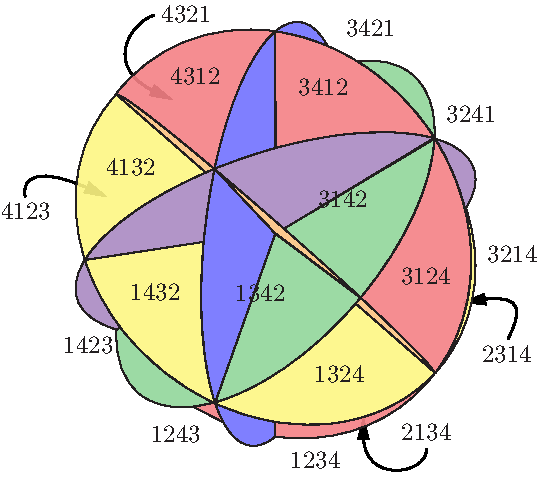
\includegraphics[height=3cm]{braidFan.pdf}
&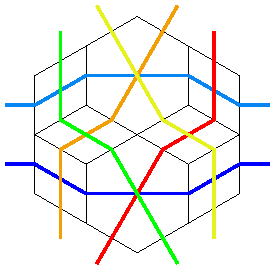
\includegraphics[height=3cm]{diagTer.pdf}
&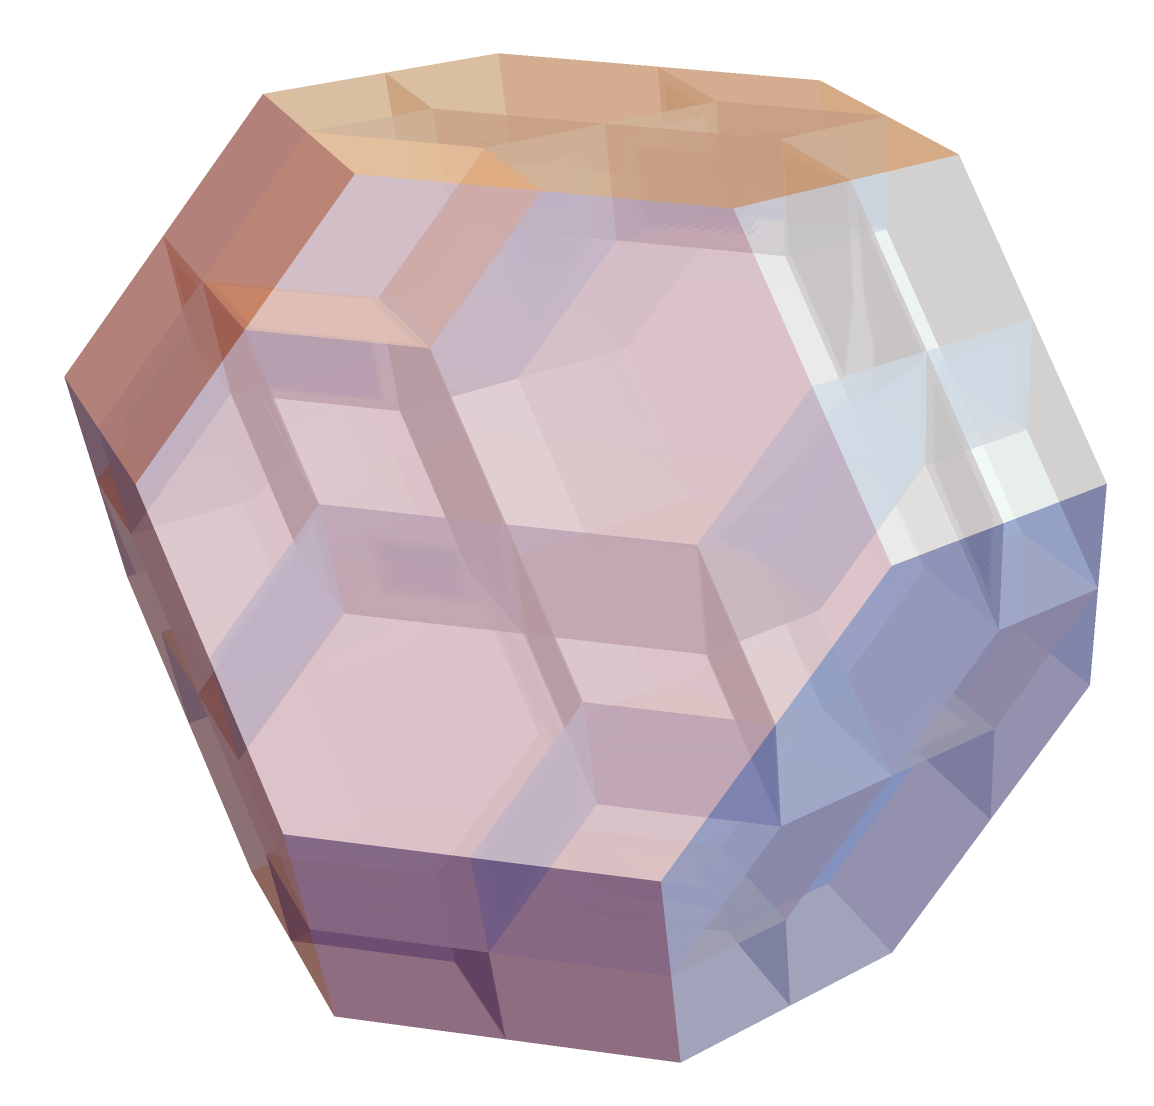
\includegraphics[height=3cm]{diagonalPermutahedronGuillaume.png} \\
\footnotesize \copyright V. Pilaud & &\footnotesize \copyright G. Laplante-Anfossi
\end{tabular}  
\begin{center}
\resizebox{0.6\textwidth}{!}{
\begin{tikzpicture}
\node (min) at (0,0){
\begin{tikzpicture}[scale=0.3, inner sep=1pt]
\node[draw, circle] (1p){1};
\node[draw, circle, right=5pt of 1p](3p){2};
\node[draw, circle, right=5pt of 3p](2p){3};
\end{tikzpicture}};
\node[above left=1cm of min.north] (3) {
\begin{tikzpicture}[scale=0.3, inner sep=1pt]
\node[draw, circle] (1p){2};
\node[draw, circle, above=5pt of 1p](3p){3};
\node[draw, circle, right=5pt of 1p](2p){1};
\draw[very thick, blue] (1p)--(3p);
\end{tikzpicture}};
\node[above right=1cm of min.north] (4) {
\begin{tikzpicture}[scale=0.3, inner sep=1pt]
\node[draw, circle] (1p){1};
\node[draw, circle, above=5pt of 1p](3p){3};
\node[draw, circle, right=5pt of 1p](2p){2};
\draw[very thick, red] (1p)--(3p);
\end{tikzpicture}};
\node[left=0.5cm of 3] (2) {
\begin{tikzpicture}[scale=0.3, inner sep=1pt]
\node[draw, circle] (1p){1};
\node[draw, circle, above=5pt of 1p](3p){2};
\node[draw, circle, right=5pt of 1p](2p){3};
\draw[very thick, blue] (1p)--(3p);
\end{tikzpicture}};
\node[left=0.5cm of 2] (1) {
\begin{tikzpicture}[scale=0.3, inner sep=1pt]
\node[draw, circle] (1p){1};
\node[draw, circle, above=5pt of 1p](3p){3};
\node[draw, circle, right=5pt of 1p](2p){2};
\draw[very thick, blue] (1p)--(3p);
\end{tikzpicture}};
\node[right=0.5cm of 4] (5) {
\begin{tikzpicture}[scale=0.3, inner sep=1pt]
\node[draw, circle] (1p){1};
\node[draw, circle, above=5pt of 1p](3p){2};
\node[draw, circle, right=5pt of 1p](2p){3};
\draw[very thick, red] (1p)--(3p);
\end{tikzpicture}};
\node[right=0.5cm of 5] (6) {
\begin{tikzpicture}[scale=0.3, inner sep=1pt]
\node[draw, circle] (1p){2};
\node[draw, circle, above=5pt of 1p](3p){3};
\node[draw, circle, right=5pt of 1p](2p){1};
\draw[very thick, red] (1p)--(3p);
\end{tikzpicture}};
\node[above=2cm of 1] (15) {
\begin{tikzpicture}[scale=0.3, inner sep=1pt]
\node[draw, circle] (1p){1};
\node[draw, circle, above left=5pt of 1p.north](2p){2};
\node[draw, circle, above right=5pt of 1p.north](3p){3};
\draw[very thick, blue] (1p)--(3p);
\draw[very thick, red] (1p)--(2p);
\end{tikzpicture}};
\node[left=0.5cm of 15] (123) {
\begin{tikzpicture}[scale=0.3, inner sep=1pt]
\node[draw, circle] (1p){1};
\node[draw, circle, above left=5pt of 1p.north](2p){2};
\node[draw, circle, above right=5pt of 1p.north](3p){3};
\draw[very thick, blue] (1p)--(3p);
\draw[very thick, blue] (1p)--(2p);
\end{tikzpicture}};
\node[right=0.5cm of 15] (26) {
\begin{tikzpicture}[scale=0.3, inner sep=1pt]
\node[draw, circle] (1p){1};
\node[draw, circle, above=5pt of 1p.north](2p){2};
\node[draw, circle, above=5pt of 2p.north](3p){3};
\draw[very thick, red] (2p)--(3p);
\draw[very thick, blue] (1p)--(2p);
\end{tikzpicture}};
\node[right=0.5cm of 26] (34) {
\begin{tikzpicture}[scale=0.3, inner sep=1pt]
\node[draw, circle] (1p){1};
\node[draw, circle, above=5pt of 1p.north](2p){3};
\node[draw, circle, above=5pt of 2p.north](3p){2};
\draw[very thick, blue] (2p)--(3p);
\draw[very thick, red] (1p)--(2p);
\end{tikzpicture}};
\node[right=0.5cm of 34] (24) {
\begin{tikzpicture}[scale=0.3, inner sep=1pt]
\node[draw, circle] (1p){1};
\node[draw, circle, above left=5pt of 1p.north](2p){2};
\node[draw, circle, above right=5pt of 1p.north](3p){3};
\draw[very thick, red] (1p)--(3p);
\draw[very thick, blue] (1p)--(2p);
\end{tikzpicture}};
\node[right=0.5cm of 24] (35) {
\begin{tikzpicture}[scale=0.3, inner sep=1pt]
\node[draw, circle] (1p){1};
\node[draw, circle, above=5pt of 1p.north](2p){2};
\node[draw, circle, above=5pt of 2p.north](3p){3};
\draw[very thick, blue] (2p)--(3p);
\draw[very thick, red] (1p)--(2p);
\end{tikzpicture}};
\node[right=0.5cm of 35] (16) {
\begin{tikzpicture}[scale=0.3, inner sep=1pt]
\node[draw, circle] (1p){1};
\node[draw, circle, above=5pt of 1p.north](2p){3};
\node[draw, circle, above=5pt of 2p.north](3p){2};
\draw[very thick, red] (2p)--(3p);
\draw[very thick, blue] (1p)--(2p);
\end{tikzpicture}};
\node[right=0.5cm of 16] (456) {
\begin{tikzpicture}[scale=0.3, inner sep=1pt]
\node[draw, circle] (1p){1};
\node[draw, circle, above left=5pt of 1p.north](2p){2};
\node[draw, circle, above right=5pt of 1p.north](3p){3};
\draw[very thick, red] (1p)--(3p);
\draw[very thick, red] (1p)--(2p);
\end{tikzpicture}};
\draw (min)--(1);
\draw (min)--(2);
\draw (min)--(3);
\draw (min)--(4);
\draw (min)--(5);
\draw (min)--(6);
\draw (123.south)--(1.north);
\draw (123.south)--(2.north);
\draw (123.south)--(3.north);
\draw (456.south)--(4.north);
\draw (456.south)--(5.north);
\draw (456.south)--(6.north);
\draw (2.north)--(26.south)--(6.north);
\draw (2.north)--(24.south)--(4.north);
\draw (1.north)--(15.south)--(5.north);
\draw (1.north)--(16.south)--(6.north);
\draw (3.north)--(34.south)--(4.north);
\draw (3.north)--(35.south)--(5.north);
\end{tikzpicture}}


\end{center}  
\end{center}
  \end{frame}


\section{The weak order and the permutohedron}\label{sect1}

\begin{frame}{Poset=partially ordered set}
\vspace{-0.5cm}
\begin{center}
\begin{tikzpicture}
\node (back) at (0,0){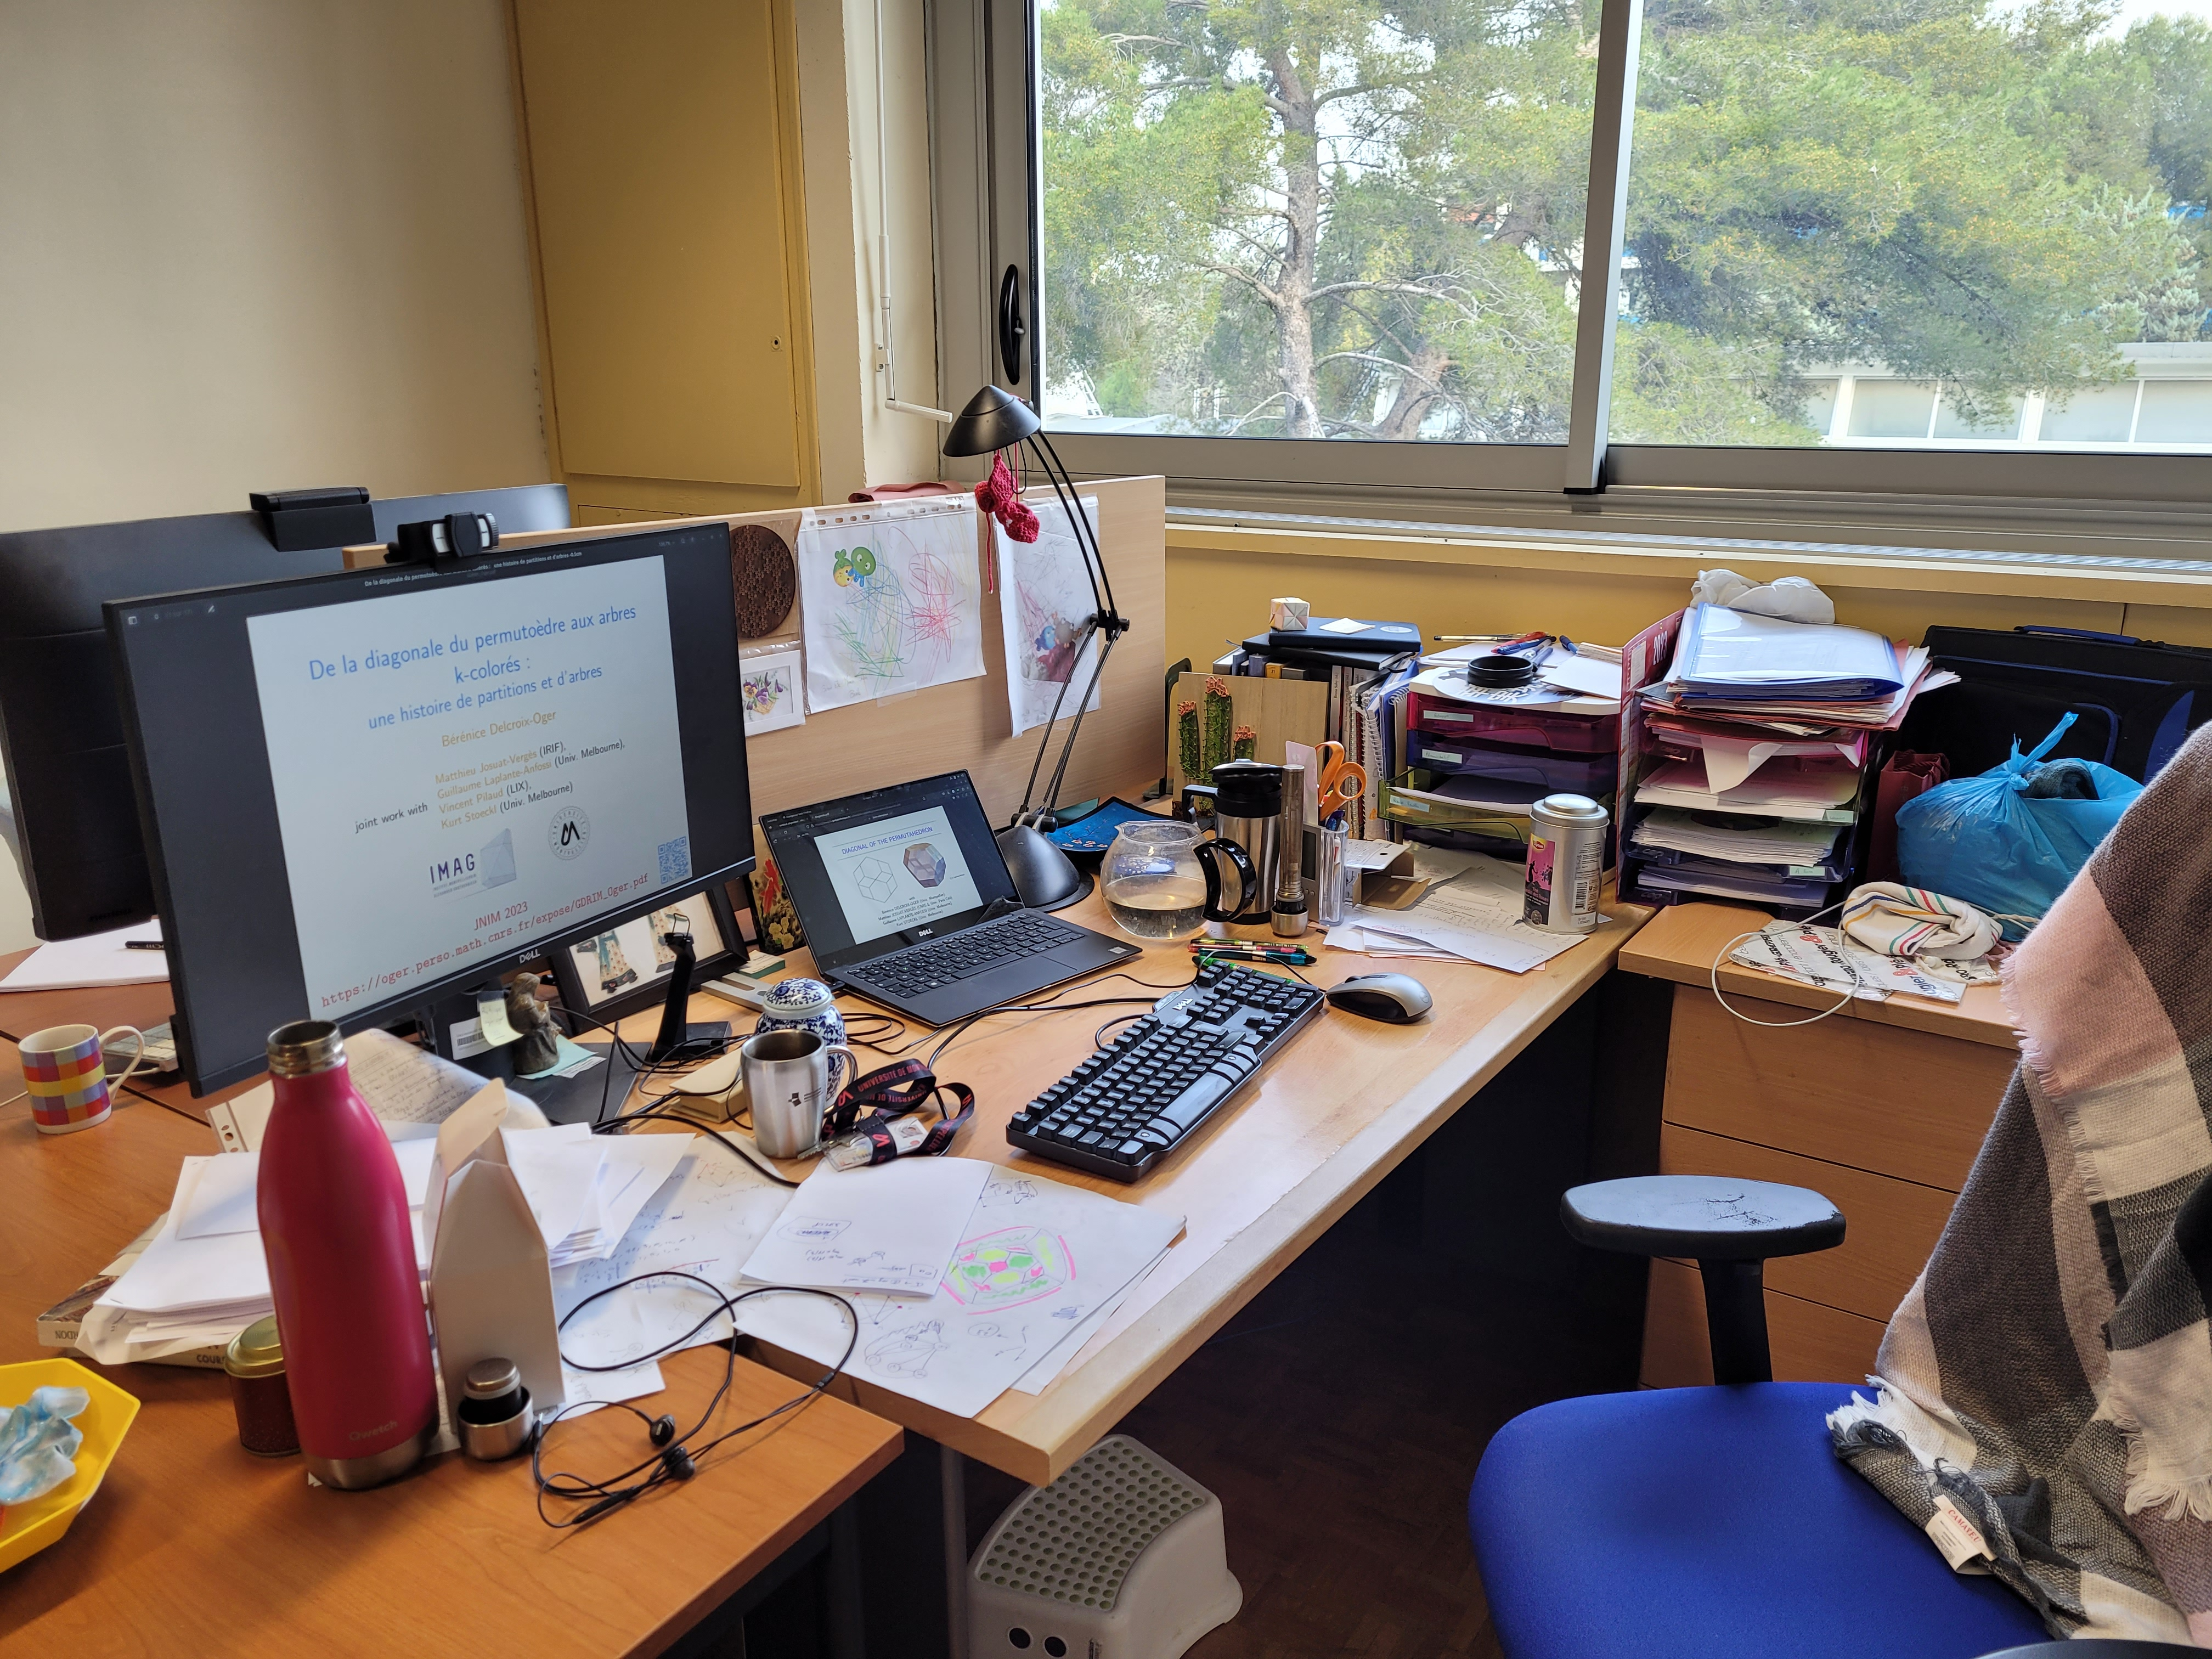
\includegraphics[width=12cm]{bureau.jpg}};
\draw<2->[line width=5pt] (1,0.5) circle (1.5cm);
\draw<2->[line width=5pt, -round cap] (0, -0.5)--(-1.5,-2);
\end{tikzpicture}
\end{center}
\end{frame}

\begin{frame}{First example of poset}
\vspace{-0.5cm}
\begin{center}
\begin{tikzpicture}[inner sep=0.15cm]
\node (back) at (0,0){
\includegraphics[width=12cm]{books.jpg}};
\onslide<2->{
\node[draw, circle, newSec, fill=newSec] (0) at(0,-3.2) {};
\node[draw, circle, newSec, fill=newSec] (1) at(1,0) {};
\node[draw, circle, newSec, fill=newSec] (2) at(0.1,0) {};
\node[draw, circle, newSec, fill=newSec] (3) at(-0.6,0) {};
\node[draw, circle, newSec, fill=newSec] (4) at(-1.2,0) {};
\node[draw, circle, newSec, fill=newSec] (5) at(-1.6,0) {};
\node[draw, circle, newSec, fill=newSec] (6) at(-2,0) {};
\node[draw, circle, newSec, fill=newSec] (7) at(-2.7,0) {};
\node[draw, circle, newSec, fill=newSec] (8) at(1.5,0) {};
\node[draw, circle, newSec, fill=newSec] (9) at(2,0) {};
\node[draw, circle, newSec, fill=newSec] (10) at(2.5,0) {};
\node[draw, circle, newSec, fill=newSec] (11) at(0.1,3.7) {};
\node[draw, circle, newSec, fill=newSec] (12) at(0.5,2.9) {};
\node[draw, circle, newSec, fill=newSec] (13) at(0,2.4) {};
\draw[white, fill=white] (2,-3.5)rectangle(5.8,-2);
\node[draw, circle, newSec, fill=newSec] (leg1) at(2.5,-2.5) {};
\node[right=1pt of leg1, anchor=west] (leg2) {= element};
\onslide<3->{
\draw[line width=5pt, part2] (2.3,-3)--(2.7,-3);
\node[anchor=west] at (2.75,-3) {= cover relation};}
\onslide<3->{\draw[line width=5pt, part2] (11)--(12)--(13);}
\onslide<5->{
\foreach \i in {1,2,...,10}
{
\draw[line width=5pt, part2] (0)--(\i);
}}
\onslide<4->{
\foreach \i in {4,6,10,8,9}
{
\draw[line width=5pt, part2] (13)--(\i);
}}}
\end{tikzpicture}
\end{center}
\end{frame}

\begin{frame}{First main example : Weak order $W_n$}
\begin{itemize}
\item To raise in the order, $\ldots ab \ldots \rightarrow \ldots ba\ldots$, with $a<b$
\end{itemize}
\begin{center}
\begin{tikzpicture}
\only<1>{\node (123) at (0,0){123};}
\only<2,3>{\node (123) at (0,0){\textcolor{newSec}{12}3};}
\only<4,5>{\node (123) at (0,0){1\textcolor{newSec}{23}};}
\only<6->{\node (123) at (0,0){123};}
\only<3>{
\node[above left=1cm of 123.north] (213){\textcolor{newSec}{21}3};
\draw[newSec] (123)--(213);}
\only<4,5, 9->{\node[above left=1cm of 123.north] (213){213};}
\only<6,7>{\node[above left=1cm of 123.north] (213){2\textcolor{newSec}{13}};}
\only<8->{\node[above left=1cm of 123.north] (213){2{13}};}
\only<4->{\draw (123)--(213);}
\only<5>{
\node[above right=1cm of 123.north] (132){1\textcolor{newSec}{32}};
\draw[newSec] (123)--(132);
}
\only<6-10,12->{
\node[above right=1cm of 123.north] (132){132};
\draw (123)--(132);
}
\only<10,11>{\node[above right=1cm of 123.north] (132){\textcolor{newSec}{13}2};
\draw (123)--(132);
}
\only<7>{
\node[above=1cm of 213.north] (231){2\textcolor{newSec}{31}};
\draw[newSec] (231)--(213);
}
\only<8>{
\node[above=1cm of 213.north] (231){\textcolor{newSec}{23}1};
}
\only<9->{
\node[above=1cm of 213.north] (231){{23}1};
}
\only<8->{
\draw (231)--(213);
}
\only<9>{
\node[above right=1cm of 231.north] (321){\textcolor{newSec}{32}1};
\draw[newSec] (231)--(321);
}
\only<10,11, 13->{
\node[above right=1cm of 231.north] (321){321};
}
\only<12>{
\node[above right=1cm of 231.north] (321){3\textcolor{newSec}{21}};
}
\only<10->{\draw (231)--(321);
}
\only<11>{
\node[above=1cm of 132.north] (312){\textcolor{newSec}{31}2};
\draw[newSec] (132)--(312);
}
\only<12>{
\node[above=1cm of 132.north] (312){3\textcolor{newSec}{12}};
\draw (132)--(312);
}
\only<13->{
\node[above=1cm of 132.north] (312){312};
\draw (132)--(312);
}
\only<12>{\draw[newSec] (312)--(321);}
\only<13->{\draw (312)--(321);}
\end{tikzpicture}
\only<14->{
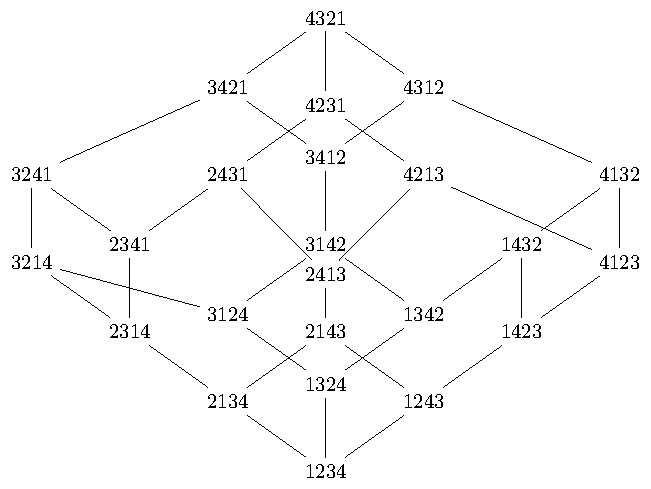
\includegraphics[height=5cm]{w4.pdf}
}
\end{center}

\end{frame}

\begin{frame}{The permutohedron = polytope with vertices labelled by permutation and edges given by the weak order}
\centering
\only<1>{
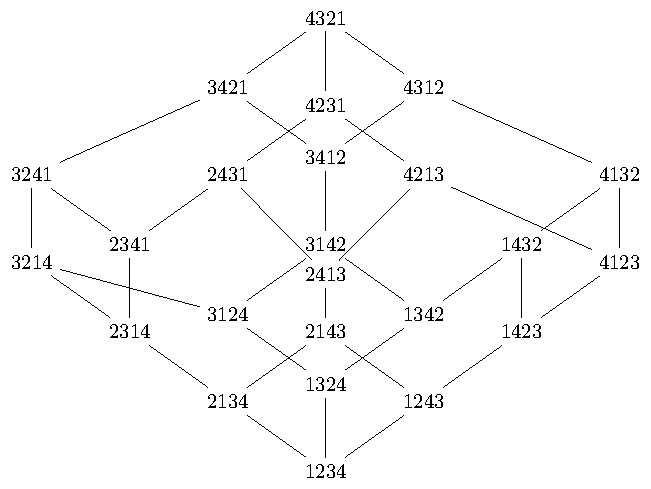
\includegraphics[height=5cm]{w4.pdf}}
\only<2->{
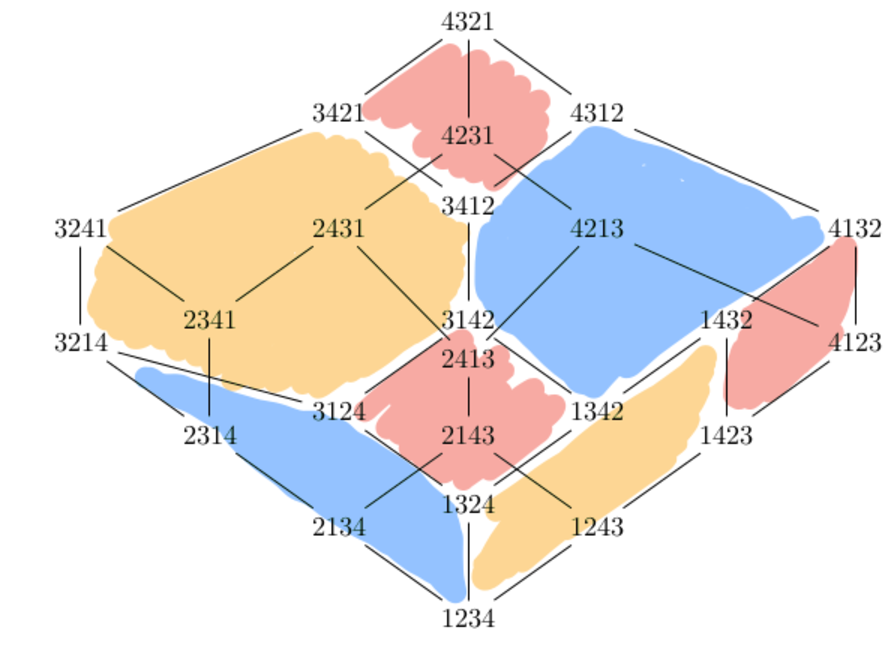
\includegraphics[height=5cm]{permcol.pdf}}
\includegraphics[height=5cm]{Permutoèdre.pdf}

\onslide<3->{
\begin{alertblock}{Short quizz :}
How many vertices does the permutohedron have ?\onslide<3->{  \textcolor{red}{$n!$}  !$\leftarrow$ \footnotesize Exclamation point}

\onslide<4->{\normalsize How many faces of dimension $n-k$ does the permutohedron have ?} \onslide<4->{\textcolor{red}{$k!S_2(n,k)$ = nb of ordered partitions in k parts of $\{1, \ldots, n\}$}}
\end{alertblock}}
\end{frame}

\begin{frame}{Labelling of the faces of the permutohedron}
\only<1>{
\begin{center}
\begin{tikzpicture}
\node (123) at (0,0) {1|2|3};
\node[above left=1cm of 123] (132) {1|3|2};
\node[above right=1cm of 123] (213) {2|1|3};
\node[above=1cm of 132] (312) {3|1|2};
\node[above=1cm of 213] (231) {2|3|1};
\node[above right=1cm of 312] (321) {3|2|1};
\draw (123) edge (132);
\draw (123) edge (213);
\draw (132) edge (312);
\draw (213) edge (231);
\draw (231) edge (321);
\draw (312) edge (321);
\end{tikzpicture}
\end{center}}

\only<2>{\begin{center}
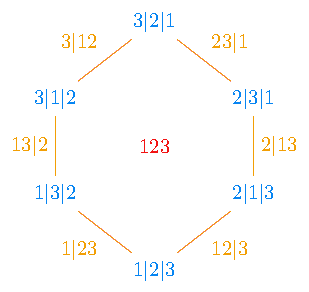
\includegraphics[height=5.5cm]{labelHex.pdf}
\end{center}}

\only<3>{
\begin{center}
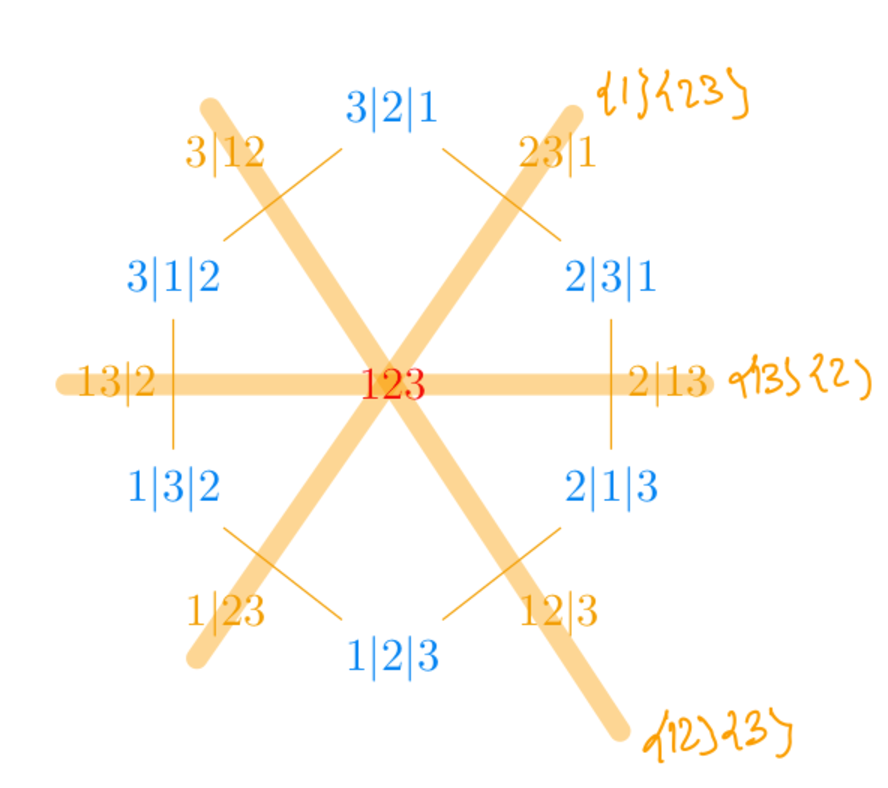
\includegraphics[height=6cm]{labelHextab.pdf}
\end{center}}

\end{frame}


\begin{frame}{Hyperplane arrangement (Thank you Sylvie !)}
Hyperplane arrangement = set of intersecting affine subspaces of codimension $1$



\begin{center}
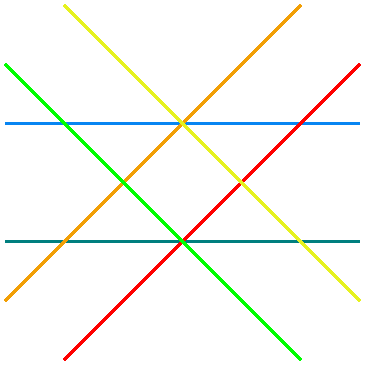
\includegraphics{arr.pdf}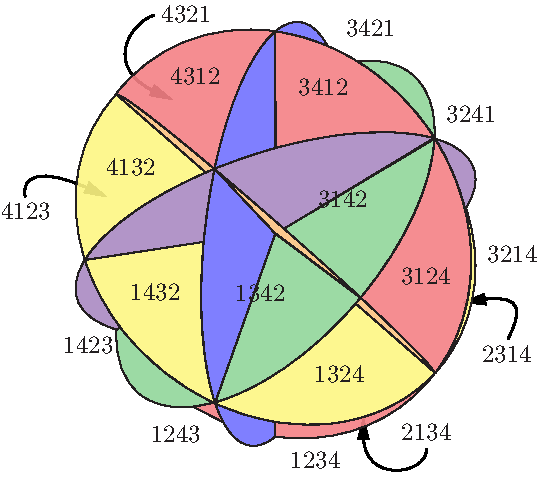
\includegraphics[height=5cm]{braidFan.pdf}
\end{center}
\begin{flushright}
\footnotesize \copyright V. Pilaud 
\end{flushright}
\end{frame}

\begin{frame}{Polytope and hyperplane arrangement}
\begin{center}
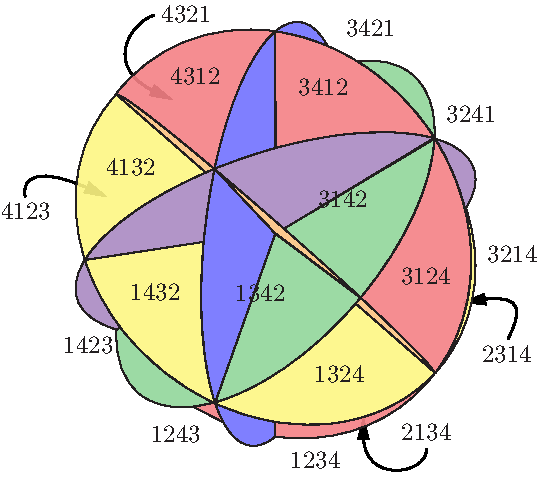
\includegraphics[height=5cm]{braidFan.pdf}
\includegraphics[height=5cm]{Permutoèdre.pdf}
\end{center}
\footnotesize \copyright V. Pilaud
\normalsize
\begin{block}{WYMR}
Number of faces of dimension $k$ = number of regions of dimension $n-k$ \textcolor{part2}{(linked with Möbius numbers of the intersection poset)}
\end{block}
\end{frame}


\section{How can we count regions of an hyperplane arrangement ?}\label{sect2}

\begin{frame}{Intersection poset}
\begin{defi}
\textcolor{newSec}{Intersection poset} = Poset of intersections of hyperplanes ordered by (reverse) inclusion
\end{defi}

\begin{center}
\begin{columns}
\begin{column}{0.5\textwidth}
\centering
\begin{tikzpicture}[scale=0.7]
\coordinate (A) at (0:2);
\coordinate (B) at (60:2);
\coordinate (C) at (120:2);
\coordinate (D) at (180:2);
\coordinate (E) at (240:2);
\coordinate (F) at (300:2);
\draw[part1, very thick]  (A)--(D);
\draw[part2, very thick]  (B)--(E);
\draw[part4, very thick]  (C)--(F);
\end{tikzpicture}
\end{column}
\begin{column}{0.5\textwidth}
\begin{tikzpicture}
\node (min) at (0,0){};
\node[above=1cm of min] (2) {
\begin{tikzpicture}[scale=0.3]
\coordinate (A) at (0:2);
\coordinate (B) at (60:2);
\coordinate (C) at (120:2);
\coordinate (D) at (180:2);
\coordinate (E) at (240:2);
\coordinate (F) at (300:2);
%\draw[part1, very thick]  (A)--(D);
\draw[part2, very thick]  (B)--(E);
%\draw[part4, very thick]  (C)--(F);
\end{tikzpicture}
};
\node[left=1cm of 2] (1) {
\begin{tikzpicture}[scale=0.3]
\coordinate (A) at (0:2);
\coordinate (B) at (60:2);
\coordinate (C) at (120:2);
\coordinate (D) at (180:2);
\coordinate (E) at (240:2);
\coordinate (F) at (300:2);
\draw[part1, very thick]  (A)--(D);
%\draw[part2, very thick]  (B)--(E);
%\draw[part4, very thick]  (C)--(F);
\end{tikzpicture}};
\node[right=1cm of 2] (3) {
\begin{tikzpicture}[scale=0.3]
\coordinate (A) at (0:2);
\coordinate (B) at (60:2);
\coordinate (C) at (120:2);
\coordinate (D) at (180:2);
\coordinate (E) at (240:2);
\coordinate (F) at (300:2);
%\draw[part1, very thick]  (A)--(D);
%\draw[part2, very thick]  (B)--(E);
\draw[part4, very thick]  (C)--(F);
\end{tikzpicture}};
\node[above=1cm of 2] (max) {
\begin{tikzpicture}[scale=0.3]
\coordinate (A) at (0:2);
\coordinate (B) at (60:2);
\coordinate (C) at (120:2);
\coordinate (D) at (180:2);
\coordinate (E) at (240:2);
\coordinate (F) at (300:2);
\draw[part1, very thick]  (A)--(D);
\draw[part2, very thick]  (B)--(E);
\draw[part4, very thick]  (C)--(F);
\end{tikzpicture}};
\draw (min)--(1);
\draw (min)--(2);
\draw (min)--(3);
\draw (max)--(1);
\draw (max)--(2);
\draw (max)--(3);
\end{tikzpicture}
\end{column}
\end{columns}
\end{center}
\end{frame}

\begin{frame}{Intersection poset : Another more complicated example}
\begin{defi}
\textcolor{newSec}{Intersection poset} = Poset of intersections of hyperplanes ordered by (reverse) inclusion
\end{defi}

\begin{center}
\begin{columns}
\begin{column}{0.3\textwidth}
\centering
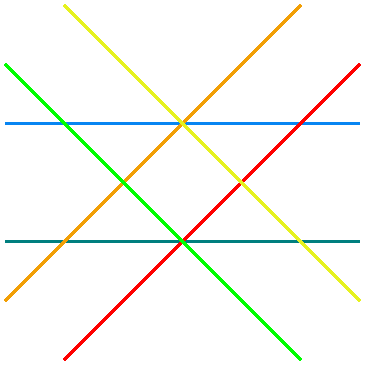
\includegraphics[width=\textwidth]{arr.pdf}
\end{column}
\begin{column}{0.7\textwidth}
\resizebox{\textwidth}{!}{
\begin{tikzpicture}
\node (min) at (0,0){};
\node[above left=1cm of min.north] (3) {
\begin{tikzpicture}[scale=0.3]
\coordinate (A) at (0:2);
\coordinate (B) at (60:2);
\coordinate (C) at (120:2);
\coordinate (D) at (180:2);
\coordinate (E) at (240:2);
\coordinate (F) at (300:2);
%\draw[part1, very thick]  (A)--(D);
\draw[part2, very thick]  (B)--(E);
%\draw[part4, very thick]  (C)--(F);
\end{tikzpicture}};
\node[above right=1cm of min.north] (4) {
\begin{tikzpicture}[scale=0.3]
\coordinate (A) at (0:2);
\coordinate (B) at (60:2);
\coordinate (C) at (120:2);
\coordinate (D) at (180:2);
\coordinate (E) at (240:2);
\coordinate (F) at (300:2);
\draw[white, very thick]  (B)--(E);
\draw[white, very thick]  (C)--(F);
\draw[teal, very thick]  (A)--(D);
\end{tikzpicture}};
\node[left=0.5cm of 3] (2) {
\begin{tikzpicture}[scale=0.3]
\coordinate (A) at (0:2);
\coordinate (B) at (60:2);
\coordinate (C) at (120:2);
\coordinate (D) at (180:2);
\coordinate (E) at (240:2);
\coordinate (F) at (300:2);
\draw[white, very thick]  (A)--(D);
\draw[white, very thick]  (B)--(E);
\draw[part4, very thick]  (C)--(F);
\end{tikzpicture}};
\node[left=0.5cm of 2] (1) {
\begin{tikzpicture}[scale=0.3]
\coordinate (A) at (0:2);
\coordinate (B) at (60:2);
\coordinate (C) at (120:2);
\coordinate (D) at (180:2);
\coordinate (E) at (240:2);
\coordinate (F) at (300:2);
\draw[white, very thick]  (B)--(E);
\draw[white, very thick]  (C)--(F);
\draw[part1, very thick]  (A)--(D);
\end{tikzpicture}};
\node[right=0.5cm of 4] (5) {
\begin{tikzpicture}[scale=0.3]
\coordinate (A) at (0:2);
\coordinate (B) at (60:2);
\coordinate (C) at (120:2);
\coordinate (D) at (180:2);
\coordinate (E) at (240:2);
\coordinate (F) at (300:2);
\draw[white, very thick]  (A)--(D);
\draw[white, very thick]  (B)--(E);
\draw[green, very thick]  (C)--(F);
\end{tikzpicture}};
\node[right=0.5cm of 5] (6) {
\begin{tikzpicture}[scale=0.3]
\coordinate (A) at (0:2);
\coordinate (B) at (60:2);
\coordinate (C) at (120:2);
\coordinate (D) at (180:2);
\coordinate (E) at (240:2);
\coordinate (F) at (300:2);
\draw[white, very thick]  (A)--(D);
\draw[white, very thick]  (C)--(F);
\draw[red, very thick]  (B)--(E);
\end{tikzpicture}};
\node[above=2cm of 1] (15) {
\begin{tikzpicture}[scale=0.3]
\coordinate (A) at (0:2);
\coordinate (B) at (60:2);
\coordinate (C) at (120:2);
\coordinate (D) at (180:2);
\coordinate (E) at (240:2);
\coordinate (F) at (300:2);
\draw[part1, very thick]  (A)--(D);
%\draw[part2, very thick]  (B)--(E);
\draw[green, very thick]  (C)--(F);
\end{tikzpicture}};
\node[left=0.5cm of 15] (123) {
\begin{tikzpicture}[scale=0.3]
\coordinate (A) at (0:2);
\coordinate (B) at (60:2);
\coordinate (C) at (120:2);
\coordinate (D) at (180:2);
\coordinate (E) at (240:2);
\coordinate (F) at (300:2);
\draw[part1, very thick]  (A)--(D);
\draw[part2, very thick]  (B)--(E);
\draw[part4, very thick]  (C)--(F);
\end{tikzpicture}
};
\node[right=0.5cm of 15] (26) {
\begin{tikzpicture}[scale=0.3]
\coordinate (A) at (0:2);
\coordinate (B) at (60:2);
\coordinate (C) at (120:2);
\coordinate (D) at (180:2);
\coordinate (E) at (240:2);
\coordinate (F) at (300:2);
%\draw[part1, very thick]  (A)--(D);
\draw[red, very thick]  (B)--(E);
\draw[part4, very thick]  (C)--(F);
\end{tikzpicture}};
\node[right=0.5cm of 26] (34) {
\begin{tikzpicture}[scale=0.3]
\coordinate (A) at (0:2);
\coordinate (B) at (60:2);
\coordinate (C) at (120:2);
\coordinate (D) at (180:2);
\coordinate (E) at (240:2);
\coordinate (F) at (300:2);
\draw[teal, very thick]  (A)--(D);
\draw[part2, very thick]  (B)--(E);
%\draw[part4, very thick]  (C)--(F);
\end{tikzpicture}};
\node[right=0.5cm of 34] (24) {
\begin{tikzpicture}[scale=0.3]
\coordinate (A) at (0:2);
\coordinate (B) at (60:2);
\coordinate (C) at (120:2);
\coordinate (D) at (180:2);
\coordinate (E) at (240:2);
\coordinate (F) at (300:2);
\draw[teal, very thick]  (A)--(D);
%\draw[part2, very thick]  (B)--(E);
\draw[part4, very thick]  (C)--(F);
\end{tikzpicture}};
\node[right=0.5cm of 24] (35) {
\begin{tikzpicture}[scale=0.3]
\coordinate (A) at (0:2);
\coordinate (B) at (60:2);
\coordinate (C) at (120:2);
\coordinate (D) at (180:2);
\coordinate (E) at (240:2);
\coordinate (F) at (300:2);
%\draw[part1, very thick]  (A)--(D);
\draw[part2, very thick]  (B)--(E);
\draw[green, very thick]  (C)--(F);
\end{tikzpicture}};
\node[right=0.5cm of 35] (16) {
\begin{tikzpicture}[scale=0.3]
\coordinate (A) at (0:2);
\coordinate (B) at (60:2);
\coordinate (C) at (120:2);
\coordinate (D) at (180:2);
\coordinate (E) at (240:2);
\coordinate (F) at (300:2);
\draw[part1, very thick]  (A)--(D);
\draw[red, very thick]  (B)--(E);
%\draw[part4, very thick]  (C)--(F);
\end{tikzpicture}};
\node[right=0.5cm of 16] (456) {
\begin{tikzpicture}[scale=0.3]
\coordinate (A) at (0:2);
\coordinate (B) at (60:2);
\coordinate (C) at (120:2);
\coordinate (D) at (180:2);
\coordinate (E) at (240:2);
\coordinate (F) at (300:2);
\draw[teal, very thick]  (A)--(D);
\draw[red, very thick]  (B)--(E);
\draw[green, very thick]  (C)--(F);
\end{tikzpicture}};
\draw (min)--(1);
\draw (min)--(2);
\draw (min)--(3);
\draw (min)--(4);
\draw (min)--(5);
\draw (min)--(6);
\draw (123.south)--(1.north);
\draw (123.south)--(2.north);
\draw (123.south)--(3.north);
\draw (456.south)--(4.north);
\draw (456.south)--(5.north);
\draw (456.south)--(6.north);
\draw (2.north)--(26.south)--(6.north);
\draw (2.north)--(24.south)--(4.north);
\draw (1.north)--(15.south)--(5.north);
\draw (1.north)--(16.south)--(6.north);
\draw (3.north)--(34.south)--(4.north);
\draw (3.north)--(35.south)--(5.north);
\end{tikzpicture}}
\end{column}
\end{columns}
\end{center}
\end{frame}

\begin{frame}{Möbius numbers}
\begin{defi}
\begin{center}
\textcolor{newSec}{Möbius function: }$\mu(x,x)=1$ and $\mu(x,y)=-\sum_{x\leq z < y} \mu(x,z) $
\end{center}
\end{defi}
\begin{center}
\only<2>{
\vspace{2cm}
\Large \textcolor{newSec}{Just like a game on an oriented graph !}}
\normalsize
\resizebox{\textwidth}{!}{
\onslide<3->{
\vspace{1cm}
\begin{tikzpicture}
\node (min) at (0,0) {$0_{\Pi_n}:=\{1\}\{2\}\{3\}$};
\node[above=10pt of min] (2)  {$\{1,3\}\{2\}$};
\node[left=80pt of 2] (1) {$\{1\}\{2,3\}$};
\node[right=80pt of 2] (3) {$\{1,2\}\{3\}$};
\node[above=10pt of 2] (max)  {$\{1,2,3\}$};
\foreach \i in {1,2,3}
{\draw (min)--(\i)--(max);}
\onslide<4->{\node[right=2pt of min, newSec] {$\mu(0_{\Pi_n},\_)=1$};}
\onslide<5->{\node[right=2pt of 1, newSec] {$\mu(0_{\Pi_n},\_)=-1$};}
\onslide<6->{\node[right=2pt of 2, newSec] {$\mu(0_{\Pi_n},\_)=-1$};
\node[right=5pt of 3, newSec] {$\mu(0_{\Pi_n},\_)=-1$};}
\onslide<7->{\node[right=5pt of max, newSec] (res){$\mu(0_{\Pi_n},\_)=2$};
\node[part3, right=10pt of res, anchor=west] (txt) {Möbius number};
\draw[->, newSec] (txt)--(res);
}
\end{tikzpicture}}}
\end{center}
\end{frame}

\begin{frame}{Zaslavsky's theorem}

Let $\mathcal{A}$ be an hyperplane arrangement and $\mathcal{I}$ be its intersection poset.
\begin{thm}[Zaslavsky, 75]
\begin{equation*}
\text{number of $k$-faces }  = \sum_{\substack{ I \leq J \in \mathcal{I} \\ \operatorname{dim}(I)=k}} |\mu(I,J)|
\end{equation*}
\end{thm}


\begin{center}
\begin{columns}
\begin{column}{0.5\textwidth}
\centering
\begin{tikzpicture}
\coordinate (A) at (0:2);
\coordinate (B) at (60:2);
\coordinate (C) at (120:2);
\coordinate (D) at (180:2);
\coordinate (E) at (240:2);
\coordinate (F) at (300:2);
\draw[part1, very thick]  (A)--(D);
\draw[part2, very thick]  (B)--(E);
\draw[part4, very thick]  (C)--(F);
\draw[very thick] (30:1)--(90:1)--(150:1)--(210:1)--(270:1)--(330:1)--cycle;
\end{tikzpicture}
\end{column}
\begin{column}{0.5\textwidth}
\centering
\begin{tikzpicture}
\node (min) at (0,0) {};
\node[above=10pt of min] (2)  {\begin{tikzpicture}[scale=0.3]
\coordinate (A) at (0:2);
\coordinate (B) at (60:2);
\coordinate (C) at (120:2);
\coordinate (D) at (180:2);
\coordinate (E) at (240:2);
\coordinate (F) at (300:2);
%\draw[part1, very thick]  (A)--(D);
\draw[part2, very thick]  (B)--(E);
%\draw[part4, very thick]  (C)--(F);
\end{tikzpicture}
};
\node[left=20pt of 2] (1) {\begin{tikzpicture}[scale=0.3]
\coordinate (A) at (0:2);
\coordinate (B) at (60:2);
\coordinate (C) at (120:2);
\coordinate (D) at (180:2);
\coordinate (E) at (240:2);
\coordinate (F) at (300:2);
\draw[part1, very thick]  (A)--(D);
%\draw[part2, very thick]  (B)--(E);
%\draw[part4, very thick]  (C)--(F);
\end{tikzpicture}};
\node[right=20pt of 2] (3) {\begin{tikzpicture}[scale=0.3]
\coordinate (A) at (0:2);
\coordinate (B) at (60:2);
\coordinate (C) at (120:2);
\coordinate (D) at (180:2);
\coordinate (E) at (240:2);
\coordinate (F) at (300:2);
%\draw[part1, very thick]  (A)--(D);
%\draw[part2, very thick]  (B)--(E);
\draw[part4, very thick]  (C)--(F);
\end{tikzpicture}};
\node[above=10pt of 2] (max)  {\begin{tikzpicture}[scale=0.3]
\coordinate (A) at (0:2);
\coordinate (B) at (60:2);
\coordinate (C) at (120:2);
\coordinate (D) at (180:2);
\coordinate (E) at (240:2);
\coordinate (F) at (300:2);
\draw[part1, very thick]  (A)--(D);
\draw[part2, very thick]  (B)--(E);
\draw[part4, very thick]  (C)--(F);
\end{tikzpicture}};
\foreach \i in {1,2,3}
\draw (min)--(\i)--(max);
\node[right=1pt of min, newSec] {$1$};
\node[right=1pt of 1, newSec] {$-1$};
\node[right=1pt of 2, newSec] {$-1$};
\node[right=1pt of 3, newSec] {$-1$};
\node[right=1pt of max, newSec] (res){$2$};
\end{tikzpicture}
\end{column}
\end{columns}
\end{center}
 
\end{frame}


\begin{frame}{In this talk : $\ell$ copies of the braid arrangement}
\begin{defi}
The \textcolor{newSec}{braid arrangement} is the hyperplane arrangement whose hyperplane satisfy equations
\begin{equation*}
H_{i,j}=\{x \in \mathbb{R}^n| x_i=x_j\}
\end{equation*}
\end{defi}

\begin{columns}
\begin{column}{0.5\textwidth}
\centering
\begin{tikzpicture}[scale=0.7]
\coordinate (A) at (0:2);
\coordinate (B) at (60:2);
\coordinate (C) at (120:2);
\coordinate (D) at (180:2);
\coordinate (E) at (240:2);
\coordinate (F) at (300:2);
\draw[part1, very thick]  (A)--(D);
\draw[part2, very thick]  (B)--(E);
\draw[part4, very thick]  (C)--(F);
\end{tikzpicture}
\end{column}
\begin{column}{0.5\textwidth}
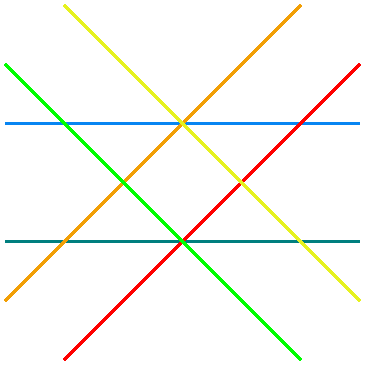
\includegraphics[width=0.7\textwidth]{arr.pdf}
\end{column}
\end{columns}


\end{frame}

\begin{frame}{Intersection poset of the braid arrangement : the partition poset $\Pi_n$}
\textcolor{newSec}{Partitions} of a set $V$ :
\begin{equation*}
\{V_1, \ldots, V_k\} \models V \Leftrightarrow V= \bigsqcup_{i=1}^k V_i, V_i\cap V_j= \emptyset \text{ for } i \neq j
\end{equation*}

Partial order on set partitions of a set $V$:
\begin{equation*}
 \textcolor{part2}{\{V'_1, \ldots, V'_p\}} \leq \textcolor{part1}{\{V_1, \ldots, V_k\}} \Leftrightarrow \textcolor{part2}{\forall i \in \{1,p\}}, \textcolor{part1}{\exists j \in \{1,k\}} \text{ s.t. } \textcolor{part2}{V'_i} \subseteq \textcolor{part1}{V_j} 
\end{equation*}
\onslide<2->{
\begin{figure}[h!]
\begin{center}
\scalebox{0.7}
{\begin{tikzpicture}[scale=0.9]
\node[draw, thick, rounded corners] (max) at (0,-5. 5) {$\{1\}\{2\}\{3\}\{4\}$};
\node[draw, thick, rounded corners, purple] (12) at (-7.5,-4) {$\{1, 2\}\{3\}\{4\}$};
\node[draw, thick, rounded corners, blue] (13) at (-4.5,-4) {$\{1, 3\}\{2\}\{4\}$};
\node[draw, thick, rounded corners, teal] (23) at (-1. 5,-4) {$\{1\}\{2, 3\}\{4\}$};
\node[draw, thick, rounded corners, green!80!black] (14) at (1.5,-4) {$\{1, 4\}\{2\}\{3\}$};
\node[draw, thick, rounded corners, orange] (24) at (4.5,-4) {$\{1\}\{2,4\}\{3\}$};
\node[draw, thick, rounded corners, red] (34) at (7.5,-4) {$\{1\}\{2\}\{3, 4\}$};
\draw[thick] (max) -- (12);
\draw[thick] (max) -- (13);
\draw[thick] (max) -- (14);
\draw[thick] (max) -- (23);
\draw[thick] (max) -- (24);
\draw[thick] (max) -- (34);
\node[draw, thick, rounded corners] (123) at (-7.5,-1. 5) {$\{1, 2, 3\}\{4\}$};
\node[draw, thick, rounded corners] (124) at (-5,-1. 5) {$\{1, 2, 4\}\{3\}$};
\node[draw, thick, rounded corners] (12d) at (-2.5,-1. 5) {$\{1, 2\}\{3, 4\}$};
\node[draw, thick, rounded corners] (13d) at (0,-1. 5) {$\{1, 3\}\{2, 4\}$};
\node[draw, thick, rounded corners] (134) at (2.5,-1. 5) {$\{1, 3, 4\}\{2\}$};
\node[draw, thick, rounded corners] (14d) at (5,-1. 5) {$\{1, 4\}\{2, 3\}$};
\node[draw, thick, rounded corners] (234) at (7.5,-1. 5) {$\{1\}\{2, 3, 4\}$};
\draw[thick, purple] (12) -- (12d);
\draw[thick, red] (34) -- (12d);
\draw[thick, blue] (13) -- (13d);
\draw[thick, orange] (24) -- (13d);
\draw[thick, green!80!black] (14) -- (14d);
\draw[thick, teal] (23) -- (14d);
\draw[thick, purple] (12) -- (123);
\draw[thick, blue] (13) -- (123);
\draw[thick, teal] (23) -- (123);
\draw[thick, purple] (12) -- (124);
\draw[thick, green!80!black] (14) -- (124);
\draw[thick, orange] (24) -- (124);
\draw[thick, blue] (13) -- (134);
\draw[thick, green!80!black] (14) -- (134);
\draw[thick, red] (34) -- (134);
\draw[thick, teal] (23) -- (234);
\draw[thick, orange] (24) -- (234);
\draw[thick, red] (34) -- (234);
\node[draw, thick, rounded corners] (min) at (0,0) {$\{1, 2, 3, 4\}$};
\draw[thick] (min) -- (12d);
\draw[thick] (min) -- (13d);
\draw[thick] (min) -- (14d);
\draw[thick] (min) -- (123);
\draw[thick] (min) -- (124);
\draw[thick] (min) -- (134);
\draw[thick] (min) -- (234);
\end{tikzpicture}}
\end{center}}
\end{figure}	
\end{frame}

\begin{frame}{Intervals and möbius numbers of the partition posets}
\begin{center}
\scalebox{0.7}
{\begin{tikzpicture}[scale=0.9]
\node[draw, thick, rounded corners] (max) at (0,-5. 5) {$\{1\}\{2\}\{3\}\{4\}$};
\node[draw, thick, rounded corners, purple] (12) at (-7.5,-4) {$\{1, 2\}\{3\}\{4\}$};
\node[draw, thick, rounded corners, blue] (13) at (-4.5,-4) {$\{1, 3\}\{2\}\{4\}$};
\node[draw, thick, rounded corners, teal] (23) at (-1. 5,-4) {$\{1\}\{2, 3\}\{4\}$};
\node[draw, thick, rounded corners, green!80!black] (14) at (1.5,-4) {$\{1, 4\}\{2\}\{3\}$};
\node[draw, thick, rounded corners, orange] (24) at (4.5,-4) {$\{1\}\{2,4\}\{3\}$};
\node[draw, thick, rounded corners, red] (34) at (7.5,-4) {$\{1\}\{2\}\{3, 4\}$};
\draw[thick] (max) -- (12);
\draw[thick] (max) -- (13);
\draw[thick] (max) -- (14);
\draw[thick] (max) -- (23);
\draw[thick] (max) -- (24);
\draw[thick] (max) -- (34);
\node[draw, thick, rounded corners] (123) at (-7.5,-1. 5) {$\{1, 2, 3\}\{4\}$};
\node[draw, thick, rounded corners] (124) at (-5,-1. 5) {$\{1, 2, 4\}\{3\}$};
\node[draw, thick, rounded corners] (12d) at (-2.5,-1. 5) {$\{1, 2\}\{3, 4\}$};
\node[draw, thick, rounded corners] (13d) at (0,-1. 5) {$\{1, 3\}\{2, 4\}$};
\node[draw, thick, rounded corners] (134) at (2.5,-1. 5) {$\{1, 3, 4\}\{2\}$};
\node[draw, thick, rounded corners] (14d) at (5,-1. 5) {$\{1, 4\}\{2, 3\}$};
\node[draw, thick, rounded corners] (234) at (7.5,-1. 5) {$\{1\}\{2, 3, 4\}$};
\draw[thick, purple] (12) -- (12d);
\draw[thick, red] (34) -- (12d);
\draw[thick, blue] (13) -- (13d);
\draw[thick, orange] (24) -- (13d);
\draw[thick, green!80!black] (14) -- (14d);
\draw[thick, teal] (23) -- (14d);
\draw[thick, purple] (12) -- (123);
\draw[thick, blue] (13) -- (123);
\draw[thick, teal] (23) -- (123);
\draw[thick, purple] (12) -- (124);
\draw[thick, green!80!black] (14) -- (124);
\draw[thick, orange] (24) -- (124);
\draw[thick, blue] (13) -- (134);
\draw[thick, green!80!black] (14) -- (134);
\draw[thick, red] (34) -- (134);
\draw[thick, teal] (23) -- (234);
\draw[thick, orange] (24) -- (234);
\draw[thick, red] (34) -- (234);
\node[draw, thick, rounded corners] (min) at (0,0) {$\{1, 2, 3, 4\}$};
\draw[thick] (min) -- (12d);
\draw[thick] (min) -- (13d);
\draw[thick] (min) -- (14d);
\draw[thick] (min) -- (123);
\draw[thick] (min) -- (124);
\draw[thick] (min) -- (134);
\draw[thick] (min) -- (234);
\end{tikzpicture}}
\end{center}
\begin{lem} For $\pi=(\pi_1, \ldots, \pi_k) \in \Pi_n$, we have:
\begin{align*}
[0_{\Pi_n},\pi] \simeq \prod_{i=1}^k \Pi_{|\pi_k|}  \hspace{1cm}
[\pi, 1_{\Pi_n}] \simeq \Pi_k \hspace{1cm} \mu(\pi, 1_{\Pi_n})=(k-1)! 
\end{align*}
\end{lem}
\end{frame}

\begin{frame}{Formula for the number of regions of the braid arrangement}

\begin{prop}
\begin{equation*}
f_{k}({\mathcal{B}_n}^\ell)=\sum_{\mathbf{F} \leq \mathbf{G}} \prod_{ G_i\in \mathbf{G}} \left( \# \mathbf{F}[G_i]-1\right)!
\end{equation*}
where $\mathbf{F} \leq \mathbf{G}$ are two partitions, $\mathbf{F}$ has $k+1$ parts and $\mathbf{F}[G_i]=\{F_j \in \mathbf{F} | F_j \subseteq G_i\}$
\end{prop}

\onslide<2->{\begin{alertblock}{Focus of the next section}
What are the underlying combinatorial object when $\ell \geq 2$ ?
\end{alertblock}}

\end{frame}



\section{The section for which you can wake up if you love graphs but hate algebra}\label{sect3}

\begin{frame}{Description of faces in terms of trees}
\begin{columns}
\begin{column}{0.4\textwidth}
\begin{tikzpicture}[scale=0.7]
\coordinate (A) at (0:2);
\coordinate (B) at (60:2);
\coordinate (C) at (120:2);
\coordinate (D) at (180:2);
\coordinate (E) at (240:2);
\coordinate (F) at (300:2);
\draw[blue, very thick]  (A)--(D);
\draw[teal, very thick]  (B)--(E);
\draw[green, very thick]  (C)--(F);
\node[blue] (123) at (0,-2){$\{1,2,3\}$};
\draw (123) edge[thick, ->, blue] (0,0);
\node[left=1pt of D, blue] (13) {$\{1,3\}\{2\}$};
\node[above left=1pt of C, blue] (12) {$\{1,2\}\{3\}$};
\node[above=1pt of B, blue] (23) {$\{1\}\{2,3\}$};
\end{tikzpicture}


\vspace{0.5cm}
\only<7->{
\begin{block}{Not every pair is possible}
\begin{center}
\centering
\sout{$(\textcolor{blue}{\{1,2\}\{3\}}, \textcolor{red}{\{1,2\}\{3\}})$}
\end{center}
\end{block}
\only<8->{
\centering
\begin{tikzpicture}
\node (12b) at (0,0) {\textcolor{blue}{1\ 2}};
\node[below=10pt of 12b] (3b) {\textcolor{blue}{3}};
\node[right=20pt of 12b] (1r){\textcolor{red}{1}};
\node[below=10pt of 1r] (23r){\textcolor{red}{23}};
\onslide<9->{
\draw (3b)edge node[midway, below]{3} (23r);
\draw (23r) edge node[midway, above, right]{2}(12b);
\draw (12b) edge node[midway, above]{1}(1r);
}
\end{tikzpicture}
\onslide<10->{\begin{tikzpicture}[scale=0.3, inner sep=1pt]
\node[draw, circle] (1p){1};
\node[draw, circle, above=5pt of 1p.north](2p){2};
\node[draw, circle, above=5pt of 2p.north](3p){3};
\node[left=5pt of 2p.west]{$=$};
\draw[very thick, red] (2p)--(3p);
\draw[very thick, blue] (1p)--(2p);
\end{tikzpicture}
}
}}
\end{column}
\begin{column}{0.6\textwidth}
\onslide<2->{
\begin{tikzpicture}[very thick]
\coordinate (C) at (180:1);
\coordinate (D) at (90:1);
\coordinate (E) at (-90:1);
\coordinate (F) at (0:1);
\coordinate (A) at ($2*(C)+(D)$); % bleu-orange
\coordinate (Ag1) at ($(A)+(C)+(D)$);
\coordinate (Ag2) at ($(A)+(C)$);
\coordinate (B) at ($2*(C)+(E)$); % teal-rouge
\coordinate (Bg1) at ($(C)+(B)$);
\coordinate (Bg2) at ($(C)+(B)+(E)$);
\coordinate (G) at ($2*(F)+(D)$);
\coordinate (Gg1) at ($(G)+(F)$);
\coordinate (Gg2) at ($(G)+(F)+(D)$);
\coordinate (H) at ($2*(F)+(E)$);
\coordinate (Hg1) at ($(H)+(F)+(E)$);
\coordinate (Hg2) at ($(H)+(F)$);
\coordinate (F1) at ($3*(E)+2*(C)$);
\coordinate (F2) at ($3*(E)+2*(F)$);
\coordinate (F3) at ($3*(D)+2*(C)$);
\coordinate (F4) at ($3*(D)+2*(F)$);
\coordinate (midb) at ($(C)+(F)+(D)$);
\draw[blue]  (Ag2)--(Gg1);
\draw[red]  (Bg1)--(Hg2);
\draw[teal]  (Bg2)--(F4);
\draw[magenta]  (F1)--(Gg2);
\draw[orange]  (Ag1)--(F2);
\draw[green]  (F3)--(Hg1);
\onslide<3->{
\node[above=2cm of midb] (eb){(\textcolor{blue}{\{1,2,3\}}, \textcolor{red}{\{1\}\{2\}\{3\}})};
\draw (eb) edge[->](midb);}
\onslide<4->{
\coordinate (midr) at ($(C)+(F)+(E)$);
\node[below=2cm of midr] (er){(\textcolor{blue}{\{1\}\{2\}\{3\}}, \textcolor{red}{\{1,2,3\}})};
\draw (er) edge[->](midr);}
\onslide<5->{
\node[right=0.5cm of F,text width=2.5cm] (ef){(\textcolor{blue}{\{1,2\}\{3\}}, \textcolor{red}{\{1\}\{2,3\}})};
\draw (ef) edge[->](F);
}
\onslide<6->{
\node[below=1.5cm of H,text width=2cm, anchor=west] (eh){(\textcolor{blue}{\{1,2\}\{3\}}, \textcolor{red}{\{1, 3\}\{2\}})};
\draw (eh) edge[->](H);
}
\end{tikzpicture}}
\end{column}
\end{columns}


\end{frame}

\begin{frame}{From intersections of hyperplanes to coloured forests}
\begin{block}{Intersection of hyperplanes}
Each intersection is a forest of edge-coloured rooted trees s.t.: 
\begin{itemize}
\item there are $\ell$ different colours of edges and $1$ is a root 
\item a child edge does not have the same colour as its parent.
\end{itemize}
\end{block}

\begin{center}
\only<1>{
\resizebox{0.8\textwidth}{!}{
\begin{tikzpicture}
\node (min) at (0,0){};
\node[above left=1cm of min.north] (3) {
\begin{tikzpicture}[scale=0.3]
\coordinate (A) at (0:2);
\coordinate (B) at (60:2);
\coordinate (C) at (120:2);
\coordinate (D) at (180:2);
\coordinate (E) at (240:2);
\coordinate (F) at (300:2);
%\draw[blue, very thick]  (A)--(D);
\draw[teal, very thick]  (B)--(E);
%\draw[part4, very thick]  (C)--(F);
\end{tikzpicture}};
\node[above right=1cm of min.north] (4) {
\begin{tikzpicture}[scale=0.3]
\coordinate (A) at (0:2);
\coordinate (B) at (60:2);
\coordinate (C) at (120:2);
\coordinate (D) at (180:2);
\coordinate (E) at (240:2);
\coordinate (F) at (300:2);
\draw[white, very thick]  (B)--(E);
\draw[white, very thick]  (C)--(F);
\draw[red, very thick]  (A)--(D);
\end{tikzpicture}};
\node[left=0.5cm of 3] (2) {
\begin{tikzpicture}[scale=0.3]
\coordinate (A) at (0:2);
\coordinate (B) at (60:2);
\coordinate (C) at (120:2);
\coordinate (D) at (180:2);
\coordinate (E) at (240:2);
\coordinate (F) at (300:2);
\draw[white, very thick]  (A)--(D);
\draw[white, very thick]  (B)--(E);
\draw[green, very thick]  (C)--(F);
\end{tikzpicture}};
\node[left=0.5cm of 2] (1) {
\begin{tikzpicture}[scale=0.3]
\coordinate (A) at (0:2);
\coordinate (B) at (60:2);
\coordinate (C) at (120:2);
\coordinate (D) at (180:2);
\coordinate (E) at (240:2);
\coordinate (F) at (300:2);
\draw[white, very thick]  (B)--(E);
\draw[white, very thick]  (C)--(F);
\draw[blue, very thick]  (A)--(D);
\end{tikzpicture}};
\node[right=0.5cm of 4] (5) {
\begin{tikzpicture}[scale=0.3]
\coordinate (A) at (0:2);
\coordinate (B) at (60:2);
\coordinate (C) at (120:2);
\coordinate (D) at (180:2);
\coordinate (E) at (240:2);
\coordinate (F) at (300:2);
\draw[white, very thick]  (A)--(D);
\draw[white, very thick]  (B)--(E);
\draw[orange, very thick]  (C)--(F);
\end{tikzpicture}};
\node[right=0.5cm of 5] (6) {
\begin{tikzpicture}[scale=0.3]
\coordinate (A) at (0:2);
\coordinate (B) at (60:2);
\coordinate (C) at (120:2);
\coordinate (D) at (180:2);
\coordinate (E) at (240:2);
\coordinate (F) at (300:2);
\draw[white, very thick]  (A)--(D);
\draw[white, very thick]  (C)--(F);
\draw[magenta, very thick]  (B)--(E);
\end{tikzpicture}};
\node[above=2cm of 1] (15) {
\begin{tikzpicture}[scale=0.3]
\coordinate (A) at (0:2);
\coordinate (B) at (60:2);
\coordinate (C) at (120:2);
\coordinate (D) at (180:2);
\coordinate (E) at (240:2);
\coordinate (F) at (300:2);
\draw[blue, very thick]  (A)--(D);
%\draw[part2, very thick]  (B)--(E);
\draw[orange, very thick]  (C)--(F);
\end{tikzpicture}};
\node[left=0.5cm of 15] (123) {
\begin{tikzpicture}[scale=0.3]
\coordinate (A) at (0:2);
\coordinate (B) at (60:2);
\coordinate (C) at (120:2);
\coordinate (D) at (180:2);
\coordinate (E) at (240:2);
\coordinate (F) at (300:2);
\draw[blue, very thick]  (A)--(D);
\draw[teal, very thick]  (B)--(E);
\draw[green, very thick]  (C)--(F);
\end{tikzpicture}
};
\node[right=0.5cm of 15] (26) {
\begin{tikzpicture}[scale=0.3]
\coordinate (A) at (0:2);
\coordinate (B) at (60:2);
\coordinate (C) at (120:2);
\coordinate (D) at (180:2);
\coordinate (E) at (240:2);
\coordinate (F) at (300:2);
%\draw[blue, very thick]  (A)--(D);
\draw[magenta, very thick]  (B)--(E);
\draw[green, very thick]  (C)--(F);
\end{tikzpicture}};
\node[right=0.5cm of 26] (34) {
\begin{tikzpicture}[scale=0.3]
\coordinate (A) at (0:2);
\coordinate (B) at (60:2);
\coordinate (C) at (120:2);
\coordinate (D) at (180:2);
\coordinate (E) at (240:2);
\coordinate (F) at (300:2);
\draw[red, very thick]  (A)--(D);
\draw[teal, very thick]  (B)--(E);
%\draw[part4, very thick]  (C)--(F);
\end{tikzpicture}};
\node[right=0.5cm of 34] (24) {
\begin{tikzpicture}[scale=0.3]
\coordinate (A) at (0:2);
\coordinate (B) at (60:2);
\coordinate (C) at (120:2);
\coordinate (D) at (180:2);
\coordinate (E) at (240:2);
\coordinate (F) at (300:2);
\draw[red, very thick]  (A)--(D);
%\draw[part2, very thick]  (B)--(E);
\draw[green, very thick]  (C)--(F);
\end{tikzpicture}};
\node[right=0.5cm of 24] (35) {
\begin{tikzpicture}[scale=0.3]
\coordinate (A) at (0:2);
\coordinate (B) at (60:2);
\coordinate (C) at (120:2);
\coordinate (D) at (180:2);
\coordinate (E) at (240:2);
\coordinate (F) at (300:2);
%\draw[blue, very thick]  (A)--(D);
\draw[teal, very thick]  (B)--(E);
\draw[orange, very thick]  (C)--(F);
\end{tikzpicture}};
\node[right=0.5cm of 35] (16) {
\begin{tikzpicture}[scale=0.3]
\coordinate (A) at (0:2);
\coordinate (B) at (60:2);
\coordinate (C) at (120:2);
\coordinate (D) at (180:2);
\coordinate (E) at (240:2);
\coordinate (F) at (300:2);
\draw[blue, very thick]  (A)--(D);
\draw[magenta, very thick]  (B)--(E);
%\draw[part4, very thick]  (C)--(F);
\end{tikzpicture}};
\node[right=0.5cm of 16] (456) {
\begin{tikzpicture}[scale=0.3]
\coordinate (A) at (0:2);
\coordinate (B) at (60:2);
\coordinate (C) at (120:2);
\coordinate (D) at (180:2);
\coordinate (E) at (240:2);
\coordinate (F) at (300:2);
\draw[red, very thick]  (A)--(D);
\draw[magenta, very thick]  (B)--(E);
\draw[orange, very thick]  (C)--(F);
\end{tikzpicture}};
\draw (min)--(1);
\draw (min)--(2);
\draw (min)--(3);
\draw (min)--(4);
\draw (min)--(5);
\draw (min)--(6);
\draw (123.south)--(1.north);
\draw (123.south)--(2.north);
\draw (123.south)--(3.north);
\draw (456.south)--(4.north);
\draw (456.south)--(5.north);
\draw (456.south)--(6.north);
\draw (2.north)--(26.south)--(6.north);
\draw (2.north)--(24.south)--(4.north);
\draw (1.north)--(15.south)--(5.north);
\draw (1.north)--(16.south)--(6.north);
\draw (3.north)--(34.south)--(4.north);
\draw (3.north)--(35.south)--(5.north);
\end{tikzpicture}}}
\only<2>{\resizebox{0.8\textwidth}{!}{
\begin{tikzpicture}
\node (min) at (0,0){
\begin{tikzpicture}[scale=0.3, inner sep=1pt]
\node[draw, circle] (1p){1};
\node[draw, circle, right=5pt of 1p](3p){2};
\node[draw, circle, right=5pt of 3p](2p){3};
\end{tikzpicture}};
\node[above left=1cm of min.north] (3) {
\begin{tikzpicture}[scale=0.3, inner sep=1pt]
\node[draw, circle] (1p){2};
\node[draw, circle, above=5pt of 1p](3p){3};
\node[draw, circle, right=5pt of 1p](2p){1};
\draw[very thick, blue] (1p)--(3p);
\end{tikzpicture}};
\node[above right=1cm of min.north] (4) {
\begin{tikzpicture}[scale=0.3, inner sep=1pt]
\node[draw, circle] (1p){1};
\node[draw, circle, above=5pt of 1p](3p){3};
\node[draw, circle, right=5pt of 1p](2p){2};
\draw[very thick, red] (1p)--(3p);
\end{tikzpicture}};
\node[left=0.5cm of 3] (2) {
\begin{tikzpicture}[scale=0.3, inner sep=1pt]
\node[draw, circle] (1p){1};
\node[draw, circle, above=5pt of 1p](3p){2};
\node[draw, circle, right=5pt of 1p](2p){3};
\draw[very thick, blue] (1p)--(3p);
\end{tikzpicture}};
\node[left=0.5cm of 2] (1) {
\begin{tikzpicture}[scale=0.3, inner sep=1pt]
\node[draw, circle] (1p){1};
\node[draw, circle, above=5pt of 1p](3p){3};
\node[draw, circle, right=5pt of 1p](2p){2};
\draw[very thick, blue] (1p)--(3p);
\end{tikzpicture}};
\node[right=0.5cm of 4] (5) {
\begin{tikzpicture}[scale=0.3, inner sep=1pt]
\node[draw, circle] (1p){1};
\node[draw, circle, above=5pt of 1p](3p){2};
\node[draw, circle, right=5pt of 1p](2p){3};
\draw[very thick, red] (1p)--(3p);
\end{tikzpicture}};
\node[right=0.5cm of 5] (6) {
\begin{tikzpicture}[scale=0.3, inner sep=1pt]
\node[draw, circle] (1p){2};
\node[draw, circle, above=5pt of 1p](3p){3};
\node[draw, circle, right=5pt of 1p](2p){1};
\draw[very thick, red] (1p)--(3p);
\end{tikzpicture}};
\node[above=2cm of 1] (15) {
\begin{tikzpicture}[scale=0.3, inner sep=1pt]
\node[draw, circle] (1p){1};
\node[draw, circle, above left=5pt of 1p.north](2p){2};
\node[draw, circle, above right=5pt of 1p.north](3p){3};
\draw[very thick, blue] (1p)--(3p);
\draw[very thick, red] (1p)--(2p);
\end{tikzpicture}};
\node[left=0.5cm of 15] (123) {
\begin{tikzpicture}[scale=0.3, inner sep=1pt]
\node[draw, circle] (1p){1};
\node[draw, circle, above left=5pt of 1p.north](2p){2};
\node[draw, circle, above right=5pt of 1p.north](3p){3};
\draw[very thick, blue] (1p)--(3p);
\draw[very thick, blue] (1p)--(2p);
\end{tikzpicture}};
\node[right=0.5cm of 15] (26) {
\begin{tikzpicture}[scale=0.3, inner sep=1pt]
\node[draw, circle] (1p){1};
\node[draw, circle, above=5pt of 1p.north](2p){2};
\node[draw, circle, above=5pt of 2p.north](3p){3};
\draw[very thick, red] (2p)--(3p);
\draw[very thick, blue] (1p)--(2p);
\end{tikzpicture}};
\node[right=0.5cm of 26] (34) {
\begin{tikzpicture}[scale=0.3, inner sep=1pt]
\node[draw, circle] (1p){1};
\node[draw, circle, above=5pt of 1p.north](2p){3};
\node[draw, circle, above=5pt of 2p.north](3p){2};
\draw[very thick, blue] (2p)--(3p);
\draw[very thick, red] (1p)--(2p);
\end{tikzpicture}};
\node[right=0.5cm of 34] (24) {
\begin{tikzpicture}[scale=0.3, inner sep=1pt]
\node[draw, circle] (1p){1};
\node[draw, circle, above left=5pt of 1p.north](2p){2};
\node[draw, circle, above right=5pt of 1p.north](3p){3};
\draw[very thick, red] (1p)--(3p);
\draw[very thick, blue] (1p)--(2p);
\end{tikzpicture}};
\node[right=0.5cm of 24] (35) {
\begin{tikzpicture}[scale=0.3, inner sep=1pt]
\node[draw, circle] (1p){1};
\node[draw, circle, above=5pt of 1p.north](2p){2};
\node[draw, circle, above=5pt of 2p.north](3p){3};
\draw[very thick, blue] (2p)--(3p);
\draw[very thick, red] (1p)--(2p);
\end{tikzpicture}};
\node[right=0.5cm of 35] (16) {
\begin{tikzpicture}[scale=0.3, inner sep=1pt]
\node[draw, circle] (1p){1};
\node[draw, circle, above=5pt of 1p.north](2p){3};
\node[draw, circle, above=5pt of 2p.north](3p){2};
\draw[very thick, red] (2p)--(3p);
\draw[very thick, blue] (1p)--(2p);
\end{tikzpicture}};
\node[right=0.5cm of 16] (456) {
\begin{tikzpicture}[scale=0.3, inner sep=1pt]
\node[draw, circle] (1p){1};
\node[draw, circle, above left=5pt of 1p.north](2p){2};
\node[draw, circle, above right=5pt of 1p.north](3p){3};
\draw[very thick, red] (1p)--(3p);
\draw[very thick, red] (1p)--(2p);
\end{tikzpicture}};
\draw (min)--(1);
\draw (min)--(2);
\draw (min)--(3);
\draw (min)--(4);
\draw (min)--(5);
\draw (min)--(6);
\draw (123.south)--(1.north);
\draw (123.south)--(2.north);
\draw (123.south)--(3.north);
\draw (456.south)--(4.north);
\draw (456.south)--(5.north);
\draw (456.south)--(6.north);
\draw (2.north)--(26.south)--(6.north);
\draw (2.north)--(24.south)--(4.north);
\draw (1.north)--(15.south)--(5.north);
\draw (1.north)--(16.south)--(6.north);
\draw (3.north)--(34.south)--(4.north);
\draw (3.north)--(35.south)--(5.north);
\end{tikzpicture}}
}
\end{center}
\end{frame}


\begin{frame}{Formula for the number of regions of $2$ copies of the braid arrangement}

\begin{thm}[BDO, M. Josuat-Vergès, G. Laplante-Anfossi, V. Pilaud, K. Stoeckl]
\begin{equation*}
f_{n-k_1-1, n-k_2-1}({\mathcal{B}_n}^2)=\sum_{\mathbf{F} \leq \mathbf{G}} \prod_{i \in [2]} \prod_{p \in G_i} \left( \# F_i[p]-1\right)!
\end{equation*}
where $\mathbf{F}$ and $\mathbf{G}$ are two forests of $2$-edge-coloured trees and $\# F_i = k_i+1$
\begin{equation*}
f_{n-1}({\mathcal{B}_n}^2)=(n+1)![x^n]exp\left(\sum_{m \geq 1} \frac{x^m}{m(m+1)} \binom{2m}{m} \right)  [A213507]
\end{equation*}
\begin{equation*}
f_{0}({\mathcal{B}_n}^2)=2(n+1)^{n-2} [A007334]
\end{equation*}
which admits the following refinement:
\begin{equation*}
f_{k, n-k-1}({\mathcal{B}_n}^2)=\frac{1}{k+1}\binom{n}{k}(k+1)^{n-k-1} (n-k)^k
\end{equation*}
\end{thm}

\end{frame}

\begin{frame}{Formula for the number of regions of $\ell$ copies of the braid arrangement}

\begin{thm}[BDO, M. Josuat-Vergès, G. Laplante-Anfossi, V. Pilaud, K. Stoeckl]
\begin{equation*}
f_{n-k_1-1,\ldots,  n-k_\ell-1}({\mathcal{B}_n}^\ell)=\sum_{\mathbf{F} \leq \mathbf{G}} \prod_{i \in [\ell]} \prod_{p \in G_i} \left( \# F_i[p]-1\right)!
\end{equation*}
where $\mathbf{F}$ and $\mathbf{G}$ are two forests of $\ell$-edge-coloured trees and $\# F_i = k_i+1$
\begin{equation*}
f_{n-1}({\mathcal{B}_n}^\ell)=??
\end{equation*}
\begin{equation*}
f_{0}({\mathcal{B}_n}^\ell)=\ell\left(1+(\ell-1)n\right)^{n-2}
\end{equation*}
which admits the following refinement:
\begin{equation*}
f_{k, n-k-1}({\mathcal{B}_n}^\ell)=??
\end{equation*}
\end{thm}

\onslide<2>{\centering \Large \textcolor{newSec}{Merci de votre attention !}}
\end{frame}

\end{document}